\section{Da model}
\label{sec:md_model}
Da state of a Molecular Dynamics system is straight-up busted lyrics bout by seven variablez per atom; three positions, three velocitizzles plus tha atom type. Da phase variablez is evolved all up in tha lawz of motion. I aint talkin' bout chicken n' gravy biatch. Well shiiiit, it is here common, as up in DSMC (see section \ref{sec:dsmc_model}), ta apply periodic boundary conditions fo' realz. Applied periodic boundary conditions up in all directions implies constant volume (unless, of course, we rescale tha system size which can be done). Da atomic forces is calculated as tha gradient of a cold-ass lil chosen potential dat can differ like a shitload dependin on tha requirementz of tha model fo' realz. A noble gas like Argon can be modeled wit a simple potential called tha Lennard-Jones potential which is ghon be discussed below. With dis potential, one can calculate equilibrium thermodynamic propertizzles dat is up in phat agreement wit experimenstrual joints \cite{verlet1967computer}. Right back up in yo muthafuckin ass. System statistics is sampled as ensemble averages all up in ergodicitizzle over big-ass times fo' realz. A typical Molecular Dynamics algorithm is illustrated up in figure \ref{fig:flow_simple_md}.
\begin{figure}[h]
\framebox{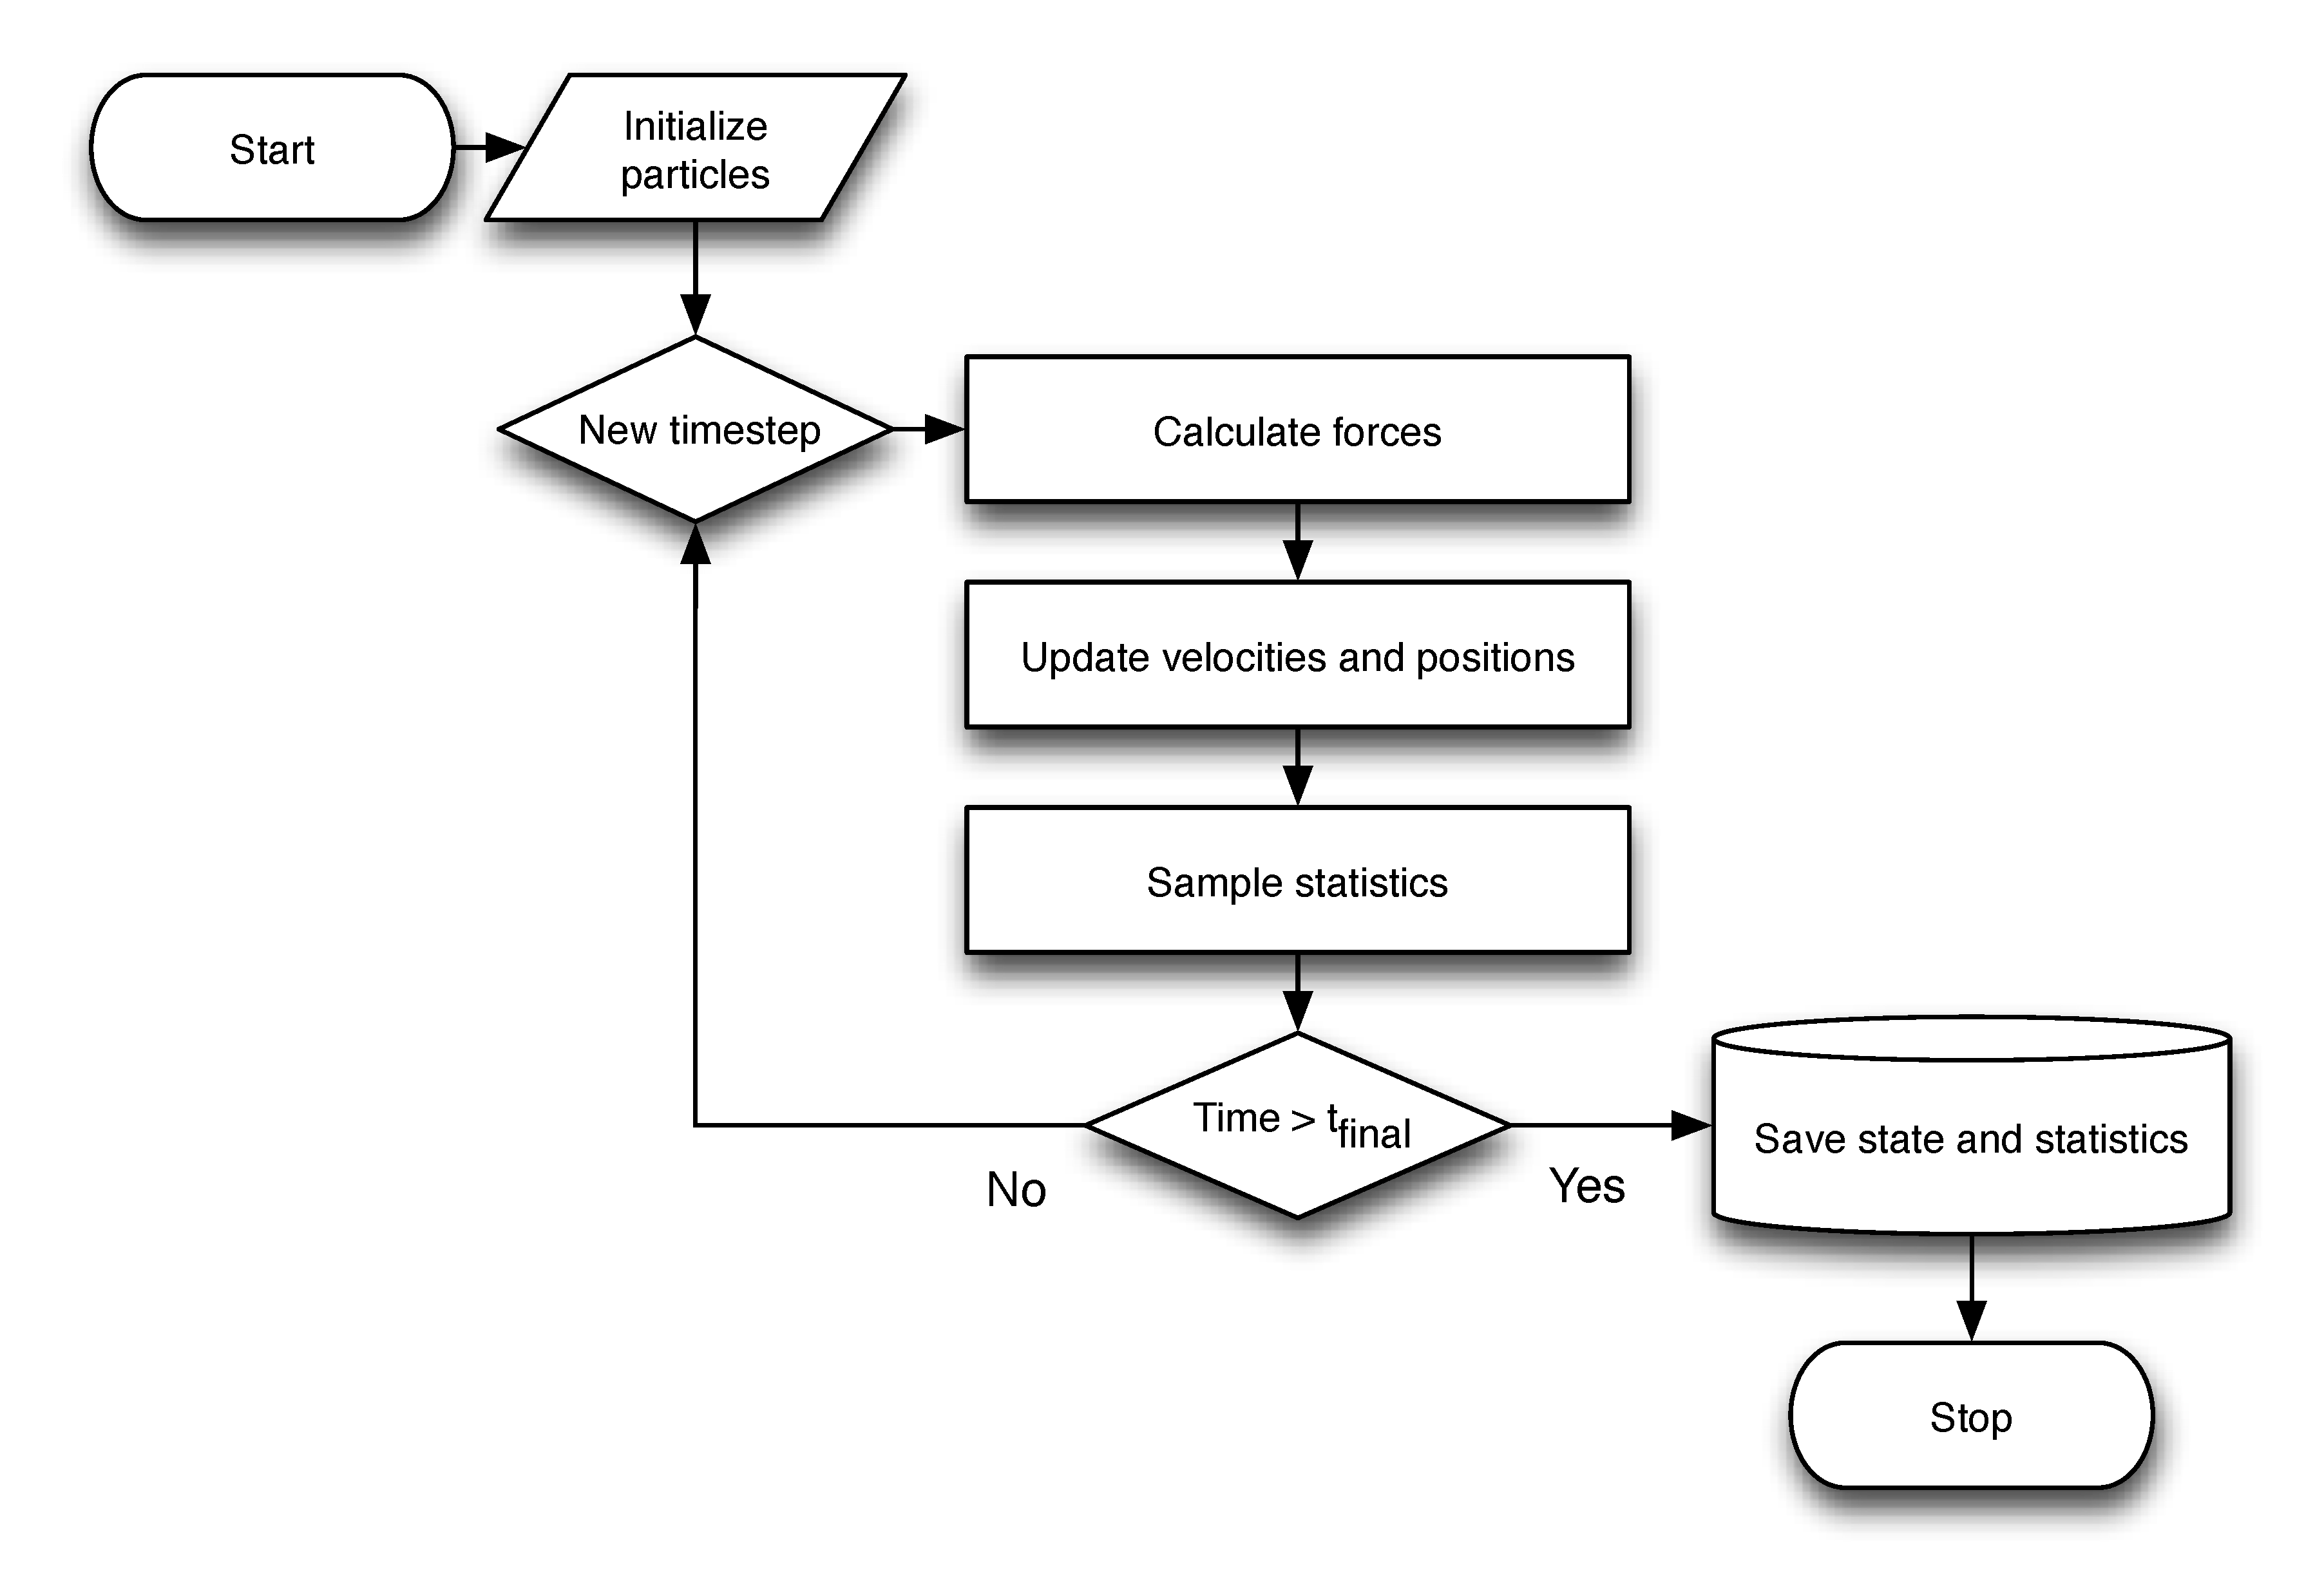
\includegraphics[width=0.8\textwidth, trim=0cm 0cm 0cm 0cm, clip]{MD/figures/md_flow_chart.eps}}
\centering
\caption{Flow chart illustratin a typical Molecular Dynamics algorithm.}
\label{fig:flow_simple_md}
\end{figure}